\documentclass[11pt,a4paper]{article}
\author{TalentSprint}
\date{}
\usepackage{graphicx}
\usepackage{verbatim}
\usepackage{array}
\usepackage{caption}
\usepackage{enumitem}
\usepackage{xcolor}
\usepackage[tikz]{bclogo}
\usepackage{textcomp}
\usepackage{listings}
\usepackage{multicol}
\usepackage{float}
\usepackage{seqsplit} 
\usepackage{setspace}
\usepackage{soul}
\usepackage{latexsym}
\lstset{language=Java,numbers=left, numberstyle=\tiny, numbersep=10pt, showstringspaces=false, breaklines=true,keepspaces=true, columns=flexible}
\usepackage{fancyhdr}
\headheight=14pt
\lhead{\nouppercase{}}
\rhead{\nouppercase{\leftmark}}

\graphicspath{{../Images/}}


\begin{comment}
\setcounter{tocdepth}{1}
\setlength\parindent{0pt}
\parskip=4pt
\def\AnswerBox{\fbox{\begin{minipage}{4in}\hfill\vspace{0.5in}\end {minipage}}}

\thispagestyle{empty}
\vspace{1.5pc}
\topskip0pt
\vspace*{\fill}
\centerline{\sc \Huge Version Control System}
\vspace{2pc}
\vspace*{\fill}
\centerline{Prepared by TalentSprint WISE Team} 
\setcounter{page}{1}
\pagestyle{fancy}
\end{comment}


%========================================================================

% Lengths and widths
\addtolength{\textwidth}{2.5cm}
\addtolength{\hoffset}{0cm}
\setlength{\headsep}{-12pt} % Reduce space between header and content
\setlength{\headheight}{85pt} % If less, LaTeX automatically increases it
\renewcommand{\footrulewidth}{2pt} % Remove footer line
\renewcommand{\headrulewidth}{1pt} % Remove header line
\renewcommand{\seqinsert}{\ifmmode\allowbreak\else\-\fi} % Hyphens in seqsplit
% This two commands together give roughly
% the right line height in the tables
\renewcommand{\arraystretch}{1.3}
\onehalfspacing



% Commands
\newcommand{\SetRowColor}[1]{\noalign{\gdef\RowColorName{#1}}\rowcolor{\RowColorName}} % Shortcut for row colour
\newcommand{\mymulticolumn}[3]{\multicolumn{#1}{>{\columncolor{white}}#2}{#3}} % For coloured multi-cols
\newcolumntype{x}[1]{>{\raggedright}p{#1}} % New column types for ragged-right paragraph columns
\newcommand{\tn}{\tabularnewline} % Required as custom column type in use

% Font and Colours
\definecolor{HeadBackground}{HTML}{333333}
\definecolor{FootBackground}{HTML}{666666}
\definecolor{TextColor}{HTML}{333333}
\definecolor{DarkBackground}{HTML}{6B8E23} %{FD1AA8}
\definecolor{LightBackground}{HTML}{E8FED8} %D3FDC8
\definecolor{tit}{HTML}{FF6600}
\renewcommand{\familydefault}{\sfdefault}
\color{TextColor}
 \headsep = 25pt
% Header and Footer
\pagestyle{fancy}
\usepackage[headheight=110pt]{geometry}
\fancyhf{}% Clear header/footer

\fancyhead[r]{
\includegraphics[width = 4cm, height = 2cm]{TS-Logo.png}\hspace{0cm}}

%=================================TITLE=====================================
\fancyhead[l]{{\bf{\textcolor{tit}{\textrm{\large{The Collection Framework}}}}}}
%===========================================================================

\renewcommand{\headrulewidth}{0.4pt}% Default \headrulewidth is 0.4pt
\renewcommand{\footrulewidth}{0.4pt}% Default \footrulewidth is 0pt

\rfoot{Page \thepage}
\lfoot{COPYRIGHT \textcopyright TALENTSPRINT, 2015. ALL RIGHTS RESERVED.}


\begin{document}

\section*{Introduction}

Arrays are used to store group of objects. Let us take an example where we want to store 100 objects of \texttt{Employee} class into an array. For this purpose, we need to create an array of \texttt{Employee} type as:
\begin{lstlisting}[numbers=none]
    Employee arr[] = new Employee[100];
\end{lstlisting}
So, here we are familiar with how to store a group of objects into an array and retrieve them again easily. But there are also certain limitations in this mechanism. They are as follows:

\begin{itemize}
\item We cannot store different class objects into the same array. The reason is that an array can store only one data type of elements.
\item Adding the objects at the end of an array is easy. But, inserting and deleting the elements in the middle of the array is difficult. In this case, we have to re-arrange all the elements of the array.
\item Retrieving the elements from an array is easy but after retrieving the elements, if we want to process them, then there are no methods available.
\end{itemize}
Due to these problems, programmers want a better mechanism to store a group of objects. The alternative is using an object to store a group of other objects. It means that we can use a class object as an array. Such an object is called ``Collection object'' or ``Container object''.

\section*{Collection Objects}
A collection in java is an object that can hold multiple objects (like an array). A collection object has a class called as ``collection class''. All these collection classes are available in the package \texttt{java.util}(util stands for Utility). A group of collection classes is called as \texttt{``Collection Framework''}.

A collection framework is a common architecture for representing and manipulating all the collections. This architecture has a set of interfaces on the top and implementing classes down the hierarchy.

All the collection classes in \texttt{java.util} package are the implementation classes of different interfaces as shown below.

\begin{table}[H]
\begin{tabular}{|l|p{7cm}|}
\hline
\textbf{Interface} & \textbf{Implementation classes} \\ \hline
Set$<$T$>$ & HastSet$<$T$>$\\
           & TreeSet$<$T$>$ \\ \hline
           & Stack$<$T$>$ \\ 
List$<$T$>$& LinkedList$<$T$>$ \\
          &  ArrayList$<$T$>$\\ 
          & Vector$<$T$>$ \\ \hline
Queue$<$T$>$ & LinkedList$<$T$>$\\ \hline
Map$<$K, V$>$ & HashMap$<$K, V$>$ \\
             & HasHable$<$K, V$>$ \\ \hline	
%Set$<$T$>$ & \parbox{4cm}{HashSet$<$T$>$ \\ LinkedHashSet$<$T$>$ TreeSet$<$T$>$} \\ \hline
%List$<$T$>$ & \parbox{4cm}{Stack$<$T$>$ \\ LinkedList$<$T$>$ \\ ArrayList$<$T$>$\\ Vector$<$T$>$} \\ \hline
%Queue$<$T$>$ & LinkedList$<$T$>$\\ \hline
%Map$<$K, V$>$ & \parbox{4cm}{HashMap$<$K, V$>$ \\HasHable$<$K, V$>$} \\ \hline

\end{tabular}
%\caption{Collection heirarchy}
\end{table}

\begin{description}
\item [Collection] is the root interface in the collection hierarchy. The items in the collection is refereed to as elements. \texttt{Collection} interface extends another interface called \texttt{Iterable}.

\item [Set] represents a group of elements arranged just like an array. The Set will grow dynamically when the elements are stored into it. A set will not allow duplicate elements. 

\item [Lists] are like sets. They store a group of elements. But lists allow duplicate values to be stored.
The subclasses of List are ordered collection of objects. List is also called sequence.

\item [Queue] represents arrangement of elements in FIFO (First In First Out) order.

\item [Map] store elements in the form of key and value pairs. If the key is provided then its corresponding value can be obtained. The keys should have unique values.
\end{description}

\begin{bclogo}[couleur=blue!5, arrondi=0.3, logo=\bclampe ]{Note}
We cannot store primitive data types in the collection objects. We can store only objects.
\end{bclogo}
\begin{figure}[H]
 \begin{center}
   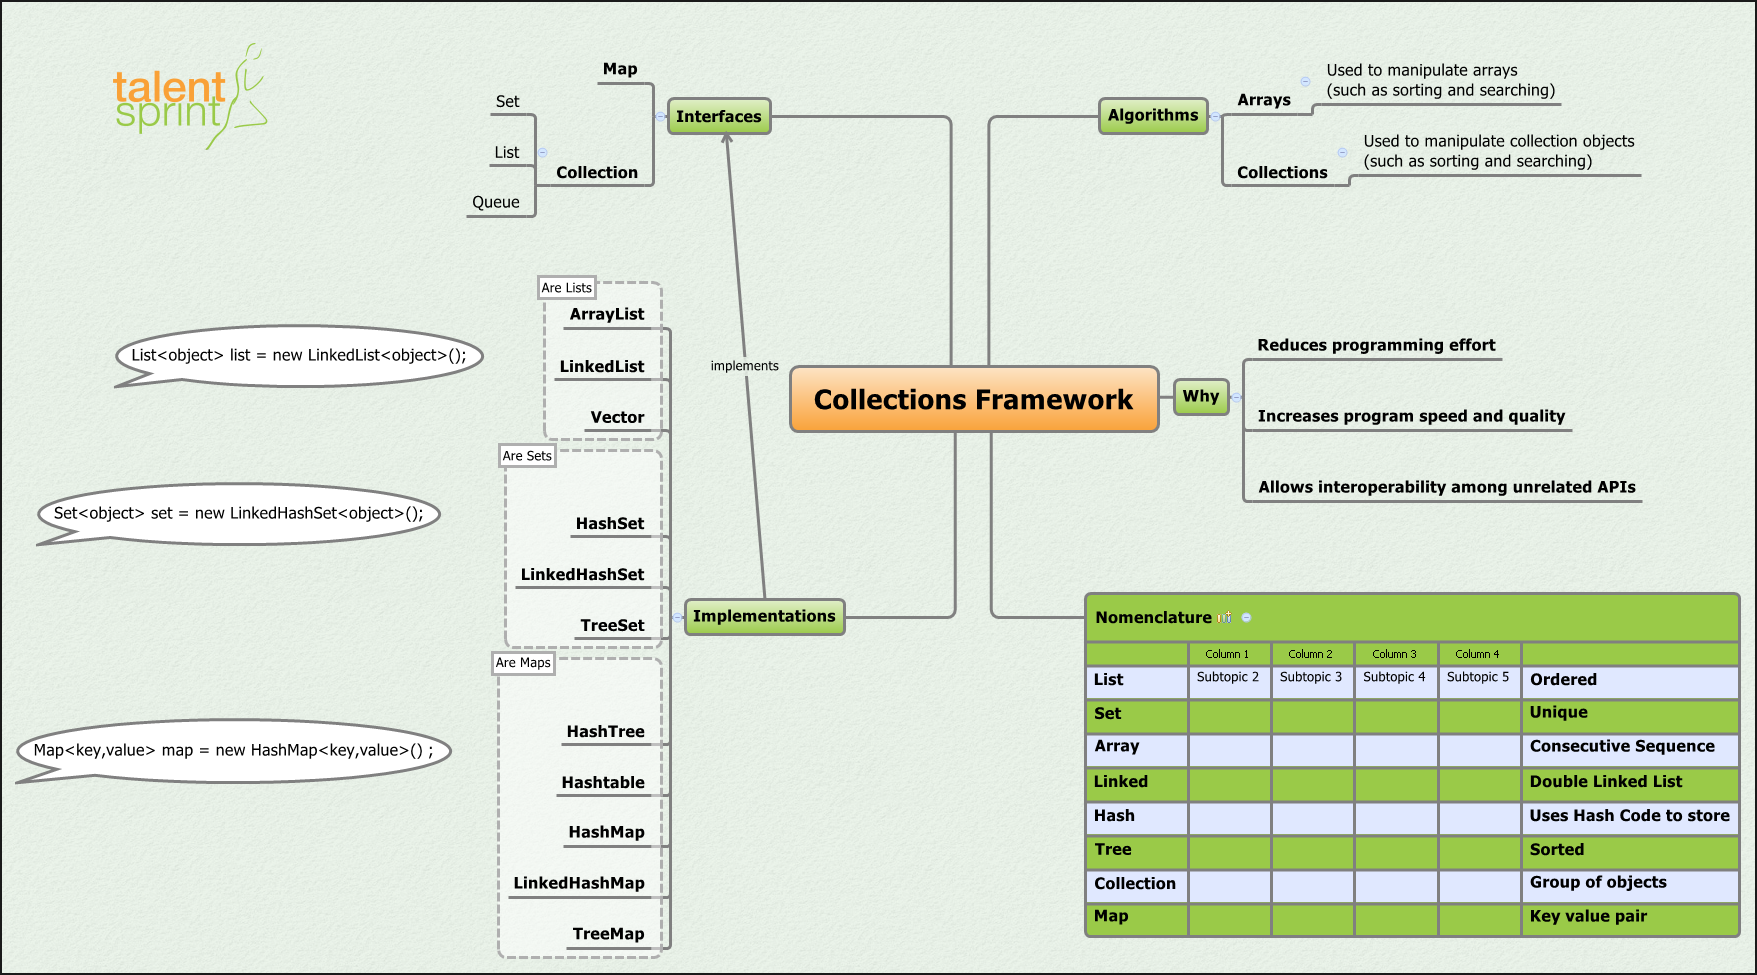
\includegraphics[angle=90,height=20cm, width=13cm]{CollectionsFramework.png}
 \end{center}
 \end{figure}
\section*{Retrieving Elements from Collections}
Following are the four ways to retrieve any element from a collection object.
\subsection*{for-each loop}
\texttt{for-each} loop is like \texttt{for} loop which repeatedly executes a group of statements for each element of the collection.
\begin{lstlisting}[numbers=none]
    for (variable-name : collection-object) {
        statement(s);
    }
\end{lstlisting}
\subsection*{Iterator}

\texttt{Iterator} is an interface that contain methods to retrieve the elements one by one from a collection object. It has three methods.
\begin{description}
\item [boolean hasNext() ] returns true if the iterator has more elements.
\item [element next() ] returns the next element in the list.
\item [void remove()] removes the last element from the collection returned by the iterator.
\end{description}

\subsection*{ListIterator}
\texttt{ListIterator} is an interface that contain methods to retrieve the elements from a collection object, both in forward and reverse directions. It has the following methods.
\begin{description}
\item [boolean hasNext()] returns true if the \texttt{ListIterator} has more elements when traversing the list  in the forward direction.
\item [boolean hasPrevious()] returns true if the \texttt{ListIterator} has more elements when traversing the list  in the reverse direction.
\item [element next() ] returns the next element in the list.
\item [element previous() ] returns the previous element in the list.
\item [void remove() ] removes the last element from the collection returned by the iterator.
\end{description}

\subsection*{Enumeration}
This interface is useful to retrieve one by one element like the iterator. It has two methods,
\begin{description}
\item [boolean hasMoreElements()] checks if the \texttt{Enumeration} has any more elements or not.
\item [element nextElement()] returns the next element that is available in\\
 \texttt{Enumeration}.
\end{description}

\section*{HashSet Class}
A \texttt{HashSet} represents a set of elements (objects). It does not guarantee the order of elements. Also it does not allow the duplicate elements to be stored.

We can write the \texttt{HashSet} class as,
\begin{lstlisting}[numbers=none]
        class HashSet<T>
\end{lstlisting}
Here, $<$T$>$ represents the generic type parameter. It represents which type of elements are being to be stored into the \texttt{HashSet}.

For example,
\begin{lstlisting}[numbers=none]
        HashSet<String> hs = new HashSet<String>();
\end{lstlisting}

\subsection*{HashSet Class Methods}
\texttt{HashSet} class provides the following methods
\begin{description}
\item [boolean add(obj)] adds an element \texttt{obj} to the \texttt{HashSet}. It returns true if the element is added to \texttt{HashSet} else it returns false. If the same element is already available in the \texttt{HashSet}, then the present element is not added.
\item [boolean remove(obj)] removes the element \texttt(obj) from the \texttt{HashSet}, if it is present. It returns true if the element is removed successfully otherwise false.
\item [void clear()] removes all the elements from the \texttt{HashSet}.
\item [boolean contains(obj)] retruns true if the \texttt{HashSet} contains the specified element \texttt{obj}.

\item [boolean isEmpty()] returns true if the \texttt{HashSet} contains no elements.
\item [int size()] returns the number of elements present in the \texttt{HashSet}.
\end{description}
\subsubsection*{Example}
Below example shows how to compare two sets, and retain the values which are common on both set objects. By calling \texttt{retainAll()} method we can retrieve common objects.
\lstinputlisting{../Code/CompareHashSets.java}

\section*{TreeSet Class}
\texttt{TreeSet} contains unique elements like HashSet. The \texttt{TreeSet} class implements \texttt{NavigableSet} interface that extends the \texttt{SortedSet} interface. \texttt{TreeSet} maintains ascending order.
\subsubsection*{Example}
The easiest way to find duplicate entries from the given array is, create \texttt{TreeSet} object and add array entries to the \texttt{TreeSet}. Since the set does not support duplicate entries, you can easily findout duplicate entries. Below example add each element to the set, and checks the returns status.
\lstinputlisting{../Code/TreesetDuplicateEntry.java}

\section*{ArrayList Class}
An \texttt{ArrayList} is like an array, which can grow in memory dynamically. It means that when we store elements into the \texttt{ArrayList}, depending on the number of elements, the memory is dynamically allocated and re-allocated to accommodate all the elements. \texttt{ArrayList} increases its size every time by 50 percent (half). 

\texttt{ArrayList} is not synchronized. But, we can use \texttt{synchronizedList()} method to synchronize the \texttt{ArrayList} as,
\begin{lstlisting}[numbers=none]
List list = Collections.synchronizedList(new ArrayList());
\end{lstlisting}
The \texttt{ArrayList}  class can be written as,
\begin{lstlisting}[numbers=none]
    class ArrayList<E>
\end{lstlisting}
For example,
\begin{lstlisting}[numbers=none]
    ArrayList<String> = new ArrayList<String>();
\end{lstlisting}

\subsection*{ArrayList Class Methods}
\begin{description}
\item [boolean add(element obj)] appends the specified element to the end of the \texttt{ArrayList}. If the element is added successfully then the preceding method returns true.
\item [void add(int position, element obj)] inserts the specified element at the specified position in the \texttt{ArrayList}.
\item [void clear()] removes all the elements from the \texttt{ArrayList}.

\item [boolean contains(Object obj)] returns true if the \texttt{ArrayList} contains the specified element.

\item [element get(int position)] returns the element available at the specified position in this \texttt{ArrayList}.

\item [int indexOf(Object obj)] returns the index of the first occurrence of the specified element in the \texttt{ArrayList}, or -1 if the \texttt{ArrayList} does not contain the element.

\item [boolean isEmpty()] returns true if this list contains no elements.
\item [int lastIndexOf(Object obj)] returns the index of the last occurrence of the specified element in this list, or -1 if this list does not contain the element.
\item [element remove(int position)] removes the element at the specified position in the \texttt{ArrayList}.
\item [boolean remove(Object obj)] removes the first occurrence of the specified element from the \texttt{ArrayList}, if it is present.

\item [element set(int index, element obj)] replaces the element at the specified position in the \texttt{ArrayList} with the specified element \texttt{obj}.
\item [int size()] returns the number of elements present in the \texttt{ArrayList}.

\item [Object\lbrack \rbrack \hspace{.3cm}toArray()] returns an array containing all of the elements in this list in proper sequence (from first to last element).

\end{description}
\subsubsection*{Example}
This example gives how to shuffle elements in the ArrayList. By calling \texttt{Collections.shuffle()} method you can shuffle the content of the ArrayList. Everytime you call \texttt{shuffle()} method, it generates different order of output.
\lstinputlisting{../Code/ShuffleArrayList.java}


\section*{Vector Class}
A \texttt{Vector} also stores elements(objects) similar to \texttt{ArrayList}, but \texttt{Vector} is synchronized. \texttt{Vector} increases its size every time by doubling it.

We can write a \texttt{Vector} class as,
\begin{lstlisting}[numbers=none]
    class Vector<E>
\end{lstlisting}
Here, \texttt{E} represents the type of elements stored into  the \texttt{Vector}.

For example,
\begin{lstlisting}[numbers=none]
    Vector<Float> v = new Vector<Float>();
\end{lstlisting}
The preceding statement creates a \texttt{Vector} object \texttt{v} which can be used to store \texttt{Float} type objects.

\subsection*{Vector Class Methods}
\begin{description}
\item [boolean add(element obj)] appends the specified element to the end of the \texttt{Vector}. If the element is added successfully then the preceding method returns true.
\item [void add(int position, element obj)] method inserts the specified element at the specified position in the \texttt{Vector}.
\item [void clear()] removes all of the elements from the \texttt{Vector}.

\item [boolean contains(Object obj)] returns true if the \texttt{Vector} contains the specified element.

\item [element get(int position)] returns the element available at the specified position in the \texttt{Vector}.

\item [int indexOf(Object obj)] returns the index of the first occurrence of the specified element in the \texttt{Vector}, or -1 if the \texttt{Vector} does not contain the element.

\item [boolean isEmpty()] returns true if this list contains no elements.
\item [int lastIndexOf(Object obj)] returns the index of the last occurrence of the specified element in this list, or -1 if this list does not contain the element.
\item [element remove(int position)] removes the element at the specified position in the \texttt{Vector}.
\item [boolean remove(Object obj)] removes the first occurrence of the specified element from the \texttt{Vector}, if it is present.

\item [element set(int index, element obj)] replaces the element at the specified position in the \texttt{Vector} with the specified element \texttt{obj}.
\item [int size()] returns the number of elements present in the \texttt{Vector}.

\item [Object\lbrack \rbrack toArray()] returns an array containing all of the elements in this list in proper sequence (from first to last element).

\item [int capacity()] returns the current capacity of the \texttt{Vector}.
\end{description}
\subsubsection*{Example}
Here, we can copy all elements of a vector object to an array. By passing an array object to copyInto() method, you can copy content of a vector object to an array and sort array in an alphabetical order by calling \texttt{Arrays.sort(array\_name)}.
\lstinputlisting{../Code/CopyVectorToArray.java}

\section*{LinkedList Class}
A \texttt{LinkedList} contains a group of elements in the form of nodes. Each node will have three fields- the data field contains data and link field contain references to previous and next nodes.

\begin{figure}[H]
\begin{center}
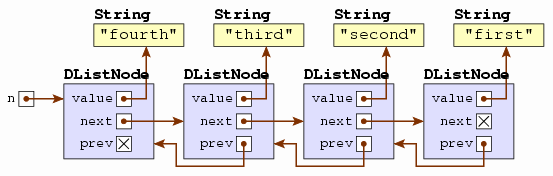
\includegraphics[scale=0.6]{linkedlist-flow.png}
%\caption{Linkedlist Work Flow}
\end{center}
\end{figure}

\texttt{LinkedList} is a convenient to store data. Inserting the elements into the \texttt{LinkedList} and removing the elements from the \texttt{LinkedList} is done quickly and takes the same amount of time.


\texttt{LinkedList} is not synchronized. But, we can use \texttt{synchronizedList()} method to synchronize the \texttt{LinkedList} as,
\begin{lstlisting}[numbers=none]
List list = Collections.synchronizedList(new LinkedList());
\end{lstlisting}

\subsection*{LinkedList Class Methods}
\begin{description}
\item [boolean add(element obj)] appends the specified element to the end of this list.
\item [void add(int position, element obj)] inserts the specified element \texttt{obj} at the specified position in this list.

\item [void addFirst(element obj)] inserts the specified element \texttt{obj} at the beginning of this list.

\item [void addLast(element obj)] appends the specified element \texttt{obj} to the end of this list.

\item [element removeFirst()] removes and returns the first element from this list.

\item [element removeLast()] removes and returns the last element from this list.

\item [element get(int position)] returns the element at the specified position in this list.

\item [element getFirst()] returns the first element in this list.

\item [element getLast()] returns the last element in this list.

\item [int size()] returns the number of elements in this list.
\end{description}
\subsubsection*{Example}
Below example shows how to iterate through LinkedList in reverse order. The method \texttt{descendingIterator()} returns an \texttt{Iterator} object with reverse order. By iterating through it, you can get the elements in the reverse order. 
\lstinputlisting{../Code/LinkedlistReverseIteration.java}

\section*{HashMap Class}
\texttt{HashMap} is a collection that store elements in the form of \texttt{key-value} pairs. If key is provided later, its corresponding value can be easily retrieved from the \texttt{HashMap}. Keys should be unique. 

\texttt{HashMap} allows null keys and null values to be stored.

\texttt{HashMap} is not synchronized. But, use synchronizedMap() to synchronize \texttt{HashMap} as,
\begin{lstlisting}[numbers=none]
Map m = Collections.synchronizedMap(new HashMap(...));
\end{lstlisting}

\subsection*{HashMap Class Methods}
\begin{description}
\item [void clear()] removes all of the mappings from this map.

\item [value get(Object key)] returns the value to which the specified key is mapped, or null if this map contains no mapping for the key.

\item [boolean isEmpty()] returns true if this map contains no key-value mappings.

\item [Set$<$K$>$ keySet()] returns a Set view of the keys contained in this map.

\item [value put(key, value)] associates the specified value with the specified key in this map.

\item [value remove(Object key)] removes the mapping for the specified key from this map if present.

\item [int size()] returns the number of key-value mappings in this map.

\item [Collection$<$V$>$ values()] returns a Collection view of the values contained in this map.
\end{description}

\subsubsection*{Example}
\lstinputlisting{../Code/GetHashMapkeys.java}


\section*{HashTable Class}
\texttt{HashTable} is similar to \texttt{HashMap} which can store elements in the form of key-value pairs. But \texttt{HashTable} is synchronized.

\texttt{HashTable} does not allow null keys or values.

\subsection*{HashTable Class Methods}
\begin{description}
\item [void clear()] clears this hashTable so that it contains no keys.

\item [Enumeration$<$V$>$	elements()] returns an enumeration of the values in this hashTable.

\item [value get(Object key)] returns the value to which the specified key is mapped, or null if this map contains no mapping for the key.

\item [boolean isEmpty()] checks if this hashTable maps no keys to values.

\item [Enumeration$<$K$>$ keys()] returns an enumeration of the keys in this hashTable.

\item [Set$<$K$>$ keySet()] returns a Set view of the keys contained in this map.

\item [value put(key, value)] maps the specified key to the specified value in this hashTable.

\item [int size()] returns the number of keys in this hashTable.

\item [Collection$<$V$>$ values()] returns a Collection view of the values contained in this map.
\end{description}

\subsubsection*{Example}
Below example shows how to get all keys as \texttt{Enumeration} object. By calling \texttt{keys()} method, we can get all keys as Enumeration object. By using Enumeration methods like \texttt{hasMoreElements()} and \texttt{nextElement()} we can read all values from HashTable.
\lstinputlisting{../Code/ReadHashtableValues.java}


\section*{StringTokenizer}
\texttt{StringTokenizer} class is useful to break a string into pieces, called `tokens'. These tokens are then stored in the \texttt{StringTokenizer} object from where they can be retrieved. 

An object to \texttt{StringTokenizer} class is,
\begin{lstlisting}[numbers=none]
StringTokenizer st = new StringTokenizer(str, ``delimiter'');
\end{lstlisting}
In the preceding statement, the actual string \texttt{str} is broken into pieces at the positions marked by a group of characters, called `delimiter'. For example, to break the string wherever a comma is found, can write as,
\begin{lstlisting}[numbers=none]
StringTokenizer st = new StringTokenizer(str, ``,'');
\end{lstlisting}
Similarly, to break the string wherever a comma or colon or both are found, we can use
\begin{lstlisting}[numbers=none]
StringTokenizer st = new StringTokenizer(str, ``,:'');
\end{lstlisting}
\subsection*{StringTokenizer Methods}
\begin{description}
\item [int countTokens()] counts and returns the number of tokens available in a \texttt{StringTokenizer} object.

\item [boolean hasMoreTokens()] checks if there are more tokens available in the \texttt{StringTokenizer} object or not. 

\item [String nextToken()] returns the next token from the \texttt{StringTokenizer}.
\end{description}
\subsubsection*{Example}
Below example shows number of token count after breaking the string by delimiter. You can get the count by using \texttt{countTokens()} method.
\lstinputlisting{../Code/CountTokens.java}


\end{document}

